\chapter{Architettura del software}
\begin{boxDef}
\textcolor{brown}{Cos'è:} si tratta dell'organizzazione del sistema o di come i componenti principali ad alto livello sono connessi tra di loro.
\end{boxDef}

\section{Elementi dell'architettura del software}
\begin{enumerate}
    \item \textbf{\textcolor{brown}{Caratteristiche architetturali:}} descrivere le qualità del software.
    \begin{enumerate}
        \item Le caratteristiche architetturali sono i requisiti non funzionali, attributi per la qualità del sistema (scalabilità, affidabilità, manutenibilità).
    \end{enumerate}
    \item \textbf{\textcolor{brown}{Decisioni architetturali:}} scelte sulla struttura del sistema che hanno un impatto significativo nel tempo.
    \begin{enumerate}
        \item Diventano vincoli che guidano lo sviluppo del software, documentati soprattutto nei progetti più grandi.
    \end{enumerate}
    \item \textbf{\textcolor{brown}{Componenti logici:}} i blocchi di costruzione di un sistema che incapsulano funzionalità specifiche, per esempio tramite directory.
    \item \textbf{\textcolor{brown}{Stili architetturali:}} la forma e struttura generale del sistema software, definendo come i componenti sono organizzati tra di loro.
    \begin{enumerate}
        \item Ad esempio i microservizi, i layer, event-driven.
    \end{enumerate}
\end{enumerate}

L'\textbf{architettura} è ad \textbf{\textcolor{blue}{alto livello}} ed ha impatto sul lungo termine, mentre invece la \textbf{progettazione} definisce la struttura di ogni classe e come interagiscono.
L'architettura riguarda la struttura del sistema, i servizi, il DB e la interazione UI, mentre il design riguarda come le funzionalità sono implementate.
Si distinguono decisioni strategiche a \textbf{lungo termine} o tattiche che sono a \textbf{breve termine} indipendenti dalle altre. Cambiare l'architettura è più costoso.

\subsection{Caratteristiche Architetturali}
Derivate dal dominio del problema e dai requisiti, dall'ambiente di sviluppo, e dalla conoscenza del dominio di lavoro.
È la parte che richiede più lavoro ed è inerente all'ambito del progetto e tendenzialmente sono \textbf{indipendenti dal dominio} di lavoro, si tratta infatti di capacità di svolgere certe operazioni, \textbf{decisioni} strutturali interne, o sulla \textbf{qualità}. Influenzano l'\textbf{architettura strutturale} e sono legate al successo. Possono essere \textbf{esplicite}, ovvero specificate direttamente nei requisiti, oppure \textbf{implicite} cioè dedotte o necessarie dal contesto.
\begin{itemize}
    \item \textbf{\textcolor{brown}{Processo:}} descrive dove il processo di sviluppo software interseca l'architettura dello stesso. Comprende modularità, facilità di testabilità, efficienza di distribuzione, facilità di estensibilità e capacità di disaccoppiamento positiva.
    \item \textbf{\textcolor{brown}{Strutturali:}} ciò che impatta la struttura interna compreso l'accoppiamento e le relazioni di integrazione. Comprende sicurezza, manutenibilità, portabilità multipiattaforma, facilità di estensione del software, localizzazione con supporto multi-lingua.
    \item \textbf{\textcolor{brown}{Operazionali:}} come le decisioni architetturali impattano sulle capacità operative del sistema. Comprende disponibilità, ripristinabilità dopo un'interruzione, robustezza in casi limite, tempo e performance, affidabilità, scalabilità utente.
    \item \textbf{\textcolor{brown}{Cross-Cutting}} decisioni che impattano sul sistema nel suo insieme. Comprende sicurezza generale, aspetti legali e leggi su dati e altro, autenticazione e autorizzazione (AAA), privacy e crittografia delle transazioni, accessibilità per tutti gli utenti, utilizzabilità.
\end{itemize}

\subsection{Decisioni Architetturali}
Per la comunicazione tra servizi si può usare il design pattern \textbf{\textcolor{blue}{Observer}}, che si può implementare in due modi diversi, tramite una \textbf{Queue} oppure con \textbf{Topic}.
Per tenere traccia delle decisioni ti utilizzano gli \textbf{ADRs (Record di Decisione Architetturali)}, ovvero un insieme di campi che compiliamo per ogni decisione.

\subsection{Componenti Logici}
Si tratta di \textbf{blocchi funzionali} del sistema all'interno del proprio dominio di lavoro. \textbf{\textcolor{blue}{Architettura logica}} significa quindi rappresentare l'interazione tra componenti, mentre \textbf{fisica} specifica come il sistema viene realizzato nella pratica.
\begin{itemize}
    \item Identificare i \textbf{componenti core}: tramite un approccio di analisi di workflow, oppure analizzando le operazioni svolte dagli attori.
    \item Assegnazione dei \textbf{requisiti} al giusto componente che è responsabile di adempirlo, evitando di creare entità che non rispettano il \textbf{SRP}.
    \item Analisi dei \textbf{ruoli} e delle \textbf{responsabilità}: assicurarmi che il componente faccia solo quello che è stato chiesto e verifica della coesione interna.
    \item Analisi delle \textbf{caratteristiche architetturali} per confermare che il componente si trova allineato con una delle caratteristiche chiave per il \textbf{successo}.
\end{itemize}

\begin{boxDef}
\textbf{\textcolor{red}{ACCOPPIAMENTO}} dei componenti si intende il grado di dipendenza tra di essi e la conoscenza che hanno gli uni degli altri, se eccessiva diff icile da mantenere. \\
\textbf{\textcolor{red}{AFFERENZA/EFFERENZA:}} fan-in/fan-out si tratta del numero di classi che dipendono dal componente e il numero di classi da cui il componente dipende.
\end{boxDef}

\subsection{Stili Architetturali}
Possono essere caratterizzati da partizionamento tecnico o di dominio, oppure modello di distribuzione.

\begin{figure}[!htb]
    \centering
    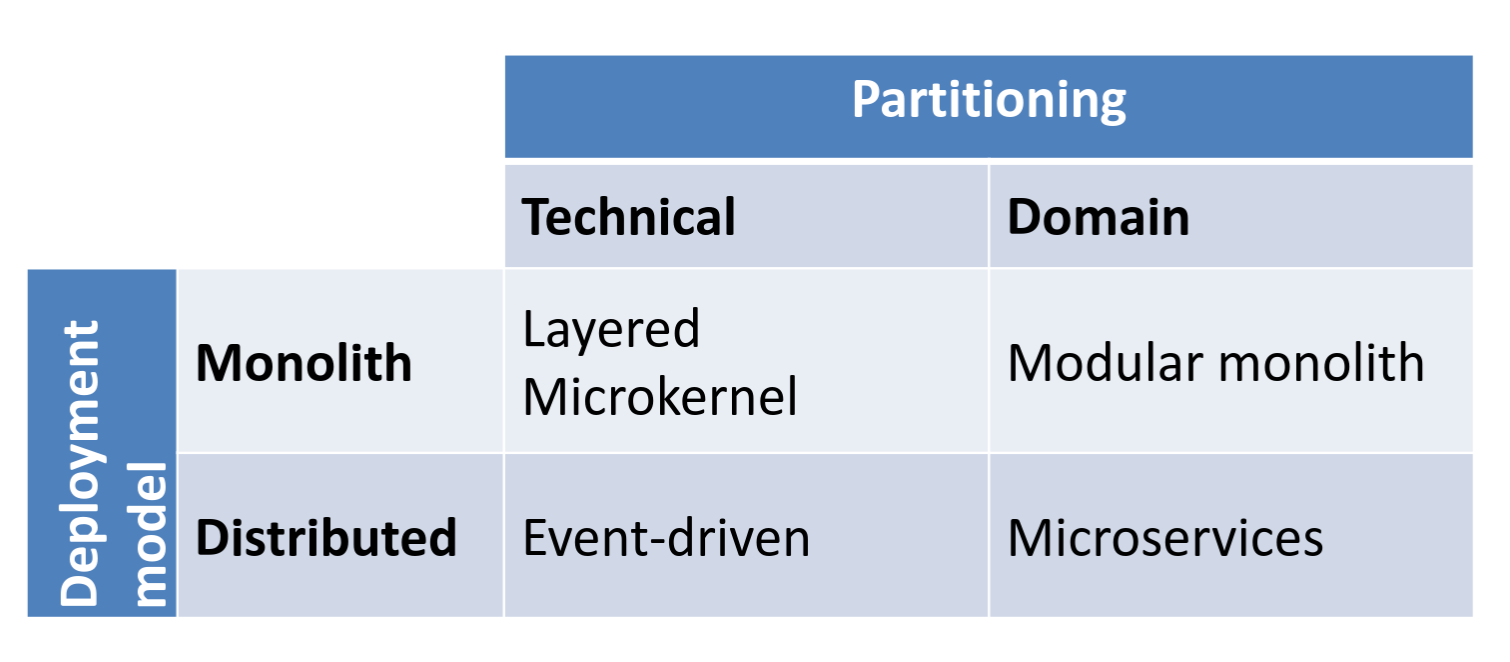
\includegraphics[width=0.6\linewidth]{Images/architettura_del_software/tabella_stili.png}
    \caption{Tabella con gli stili architetturali.}
\end{figure}

Può essere \textbf{\textcolor{forest_green}{monolitico}} se si basano su un'unica unità, altrimenti \textbf{\textcolor{forest_green}{distribuito}} se è organizzato in componenti che possono essere provati in luoghi diversi.
Il partizionamento \textbf{\textcolor{blue}{tecnico}} divide il software in pacchetti, mentre quello per dominio come dice il termine è suddiviso in moduli legati al \textbf{\textcolor{blue}{dominio}}.

\begin{itemize}
    \item Il \textbf{monolitico} è semplice, economico, più facilmente realizzabile e debuggabile, ma non è scalabile, difficile da evolvere e va ridistribuito per intero.
    \item I sistemi \textbf{distribuiti} invece sono più scalabili, modulari, resilienti, testabili e distribuibili più facilmente
    D'altra parte però sono più lenti, difficili da debuggare e risalire allo stack di errore, sono più complessi e costosi.
\end{itemize}

\subsubsection{Monoliti a Livelli}
Principalmente utilizzati quando deve entrare in produzione velocemente, oppure quando è importante separare le responsabilità rispettando \textbf{SRP} per i lavoratori che abbiamo, o ancora quando abbiamo bisogno di un prodotto facilmente estensibile.
Utilizza il paradigma di programmazione \textbf{\textcolor{blue}{MVC}} ovvero \textbf{\textcolor{blue}{Model View Controller}}. Il modello rappresenta la logica di business, la vista rappresenta l'interfaccia utente, il controller si occupa del workflow e delle funzionalità coese.

\vspace*{0.02\textheight}
I livelli partizionati sono \textbf{isolati} dagli altri, \textbf{indipendenti}, \textbf{chiusi} tra di loro e sono facilmente \textbf{rimpiazzabili}. Tuttavia esiste il modo di lasciare alcuni livelli \textbf{aperti}, creando un livello servizi quando ci sia la necessità di avere oggetti condivisi all'interno del livello di business. A livello di \textbf{architettura fisica}:
\begin{enumerate}
    \item Architettura fisica a \textbf{due strati} che separa la parte della memorizzazione dai dati dal resto, è semplice, veloce e a scalabilità e affidabilità media.
    \item  Architettura fisica a \textbf{tre strati} che separa anche la parte di presentazione web ma è la meno affidabile perché complessa nonostante sia distribuita.
    \item Architettura fisica di tipo \textbf{embedded o mobile} che contiene tutto, è il meno scalabile, limitato dalle risorse e legato molto all'implementazione.
\end{enumerate}
Questo tipo di partizionamento è velocemente \textbf{realizzabile}, \textbf{efficiente} e \textbf{ottimizzato}. Non è, però, scalabile, è difficile da testare e distribuire e rischioso.

\subsubsection{Monoliti Modulari} 
Permettono di eseguire una partizione funzionale in base al \textbf{dominio} dell'operazione, o al \textbf{sottodominio}. Dividono il progetto in moduli, ciascuno dei quali ha tre componenti di presentazione, logica di business e persistenza dei dati. I team hanno consapevolezza degli interi livelli di quel dominio.
Per mantenere i moduli modulabili bisogna mantenere le classi disaccoppiate in modo da evitare delle dipendenze indesiderate. I moduli sono considerabili ciascuno un \textbf{servizio indipendente} ma distribuiti come uno unico, ciascuno che espone le proprie \textbf{\textcolor{blue}{API}} e nasconde l'implementazione.

\subsubsection{Micorkernel} 
Permette di aggiungere i \textbf{\textcolor{blue}{plugin}} al \textbf{core} del sistema, tramite un registro di plugin usando dei contratti per eseguirli.
I plugin possono essere di tipo \textbf{monolitico} ed essere \textbf{embedded} con il core, oppure \textbf{distribuiti} ed essere anche su altre tecnologie e dispositivi \textbf{sync} o \textbf{async}.
Il core contiene un \textbf{registro} che contiene la lista dei plugin disponibili per l'esecuzione e come accedervi, quindi contratti e protocolli.
\begin{itemize}
    \item I \textbf{contratti} possono essere standard e descrivere caratteristiche comuni, oppure personalizzati e spesso richiedono un adapter per convertirli.
\end{itemize}
Viene utilizzato moltissimo perché è \textbf{scalabile}, \textbf{adattabile}, \textbf{evolvibile}, ha una struttura semplice e con il partizionamento garantisce \textbf{flessibilità}.
Gli svantaggi avvengono quando devo modificare spesso il core, quando introduco dipendenze tra i plugin o risorse condivise, ed è meno performante.

\subsubsection{Microservizi}
\begin{boxDef}
Un \textbf{\textcolor{blue}{microservizio}} è un'unità di codice single-purpose, distribuita indipendentemente.
\end{boxDef}
Le archietture di questo tipo sono distribuite, partizionate per dominio. 
\begin{itemize}
    \item \textbf{\textcolor{brown}{Granularità:}} è una delle caratteristiche più importanti perché se facciamo servizi troppo piccoli serve coordinazione, se troppo grandi perde di senso.
    \begin{itemize}
        \item \textbf{Disintegratori:} forzano a fare servizi piccoli quando il codice è volatile, può fallire, quando è scalabile o serve \textbf{ACL}.
        \item \textbf{Integratori:} forzano a fare servizi grossi, quando ci sono dipendenze di dati o tra microservizi, o in fase di commit sul \textbf{DB}.
    \end{itemize}
\end{itemize}
Il \textbf{riutilizzo} del codice in questi casi è essenziale per funzioni comuni a tutti come i logger e posso far dipendere il codice da librerie comuni più veloci, meno rischiose, ma complesse, difficili da mantenere e distribuire; oppure da servizi comuni rischiosi per errori di rete, ma implementabili in qualsiasi linguaggio.

\vspace*{0.02\textheight}
Per il flusso di lavoro e la coesione dei microservizi posso usare due metodi:
\begin{enumerate}
    \item \textbf{\textcolor{brown}{Orchestrazione:}} un broker che stabilisce la successione delle operazioni, in cui è più facile da cambiare l'ordine.
    \item \textbf{\textcolor{brown}{Coreografia:}} ogni servizio chiama il suo successore, migliori performance, scalabile ma più difficile da debuggare.
\end{enumerate}
La struttura a microservizi è più facile da \textbf{mantenere}, \textbf{testare}, \textbf{distribuire}, \textbf{evolvere}, è \textbf{scalabile} e \textbf{tollerante} agli errori. D'altra parte invece è scomoda perché più \textbf{complessa}, accoppiata al database in ogni servizio, per \textbf{problemi di rete} e richiede più team tutti \textbf{competenti} su tutto.

\subsubsection{Event-Driven}
\begin{boxDef}
\textbf{\textcolor{brown}{Eventi:}} sono avvenimenti importanti che vengono inoltrati in broadcast ai servizi listener e solo quelli interessati agiscono. Le comunicazioni sono asincrone, dato che chi genera l'evento non attende risposta, difficile la gestione dell'errore. I \textbf{messaggi} invece sono comandi diretti.
\end{boxDef}
Ci sono diversi livelli su cui valutare questo tipo di architettura:
\begin{itemize}
    \item \textbf{\textcolor{brown}{Performance:}} gli \textbf{EDA} permettono il parallelismo e l'asincrono quindi sono più veloci dei microservizi che introducono latenza.
    \item \textbf{\textcolor{brown}{Dipendenza fisica:}} gli \textbf{EDA} non hanno bisogno di esserlo, mentre i microservizi richiedono la proprietà dei dati, non la condivisione.
    \item \textbf{\textcolor{brown}{Granularità dei dati:}} i microservizi possiedono ciascuno i propri, mentre negli \textbf{EDA} si possono avere varie strutture \textbf{DB} che vedremo.
    \item \textbf{\textcolor{brown}{Granularità dei servizi:}} i microservizi sono molto specifici e fanno una funzione, mentre gli \textbf{EDA} possono essere entrambi.
    \item \textbf{\textcolor{brown}{Processamento:}} gli \textbf{EDA} si basano sull'elaborare eventi e reagire ad essi, mentre i microservizi elaborano su richiesta.
    \item \textbf{\textcolor{brown}{Comunicazione:}} gli \textbf{EDA} comunicano asincronicamente tra servizi, mentre i microservizi sono sincroni e usano \textbf{\textcolor{blue}{Rest}}.
\end{itemize}

Tra i \textbf{\textcolor{red}{vantaggi}} di un'architettura \textbf{EDA} c'è il disaccoppiamento per migliorare la \textbf{manutenzione}, la \textbf{velocità}, resistenza agli \textbf{errori} e \textbf{scalabilità}. Gli \textbf{\textcolor{red}{svantaggi}} invece includono l'\textbf{accoppiamento} con i \textbf{DB} o tra i \textbf{servizi}, la difficoltà di \textbf{testing}, \textbf{inadeguatezza} a chiamate sincrone, e la \textbf{complessità}.

\vspace*{0.02\textheight}
La \textbf{topologia} del database può essere di tipo \textbf{monolitico}, con un unico DB molto centralizzato. Oppure \textbf{partizionata} per dominio, dove ogni dominio ha il suo DB ma introduce accoppiamento tra servizi o ogni servizio ha il suo DB.
\begin{itemize}
    \item Il \textbf{\textcolor{brown}{modello broker}} ha un semplice gestore degli eventi leggero su ogni \textbf{listener} che accetta dal broker l'evento, svolge una task e risponde asincrono.
    \begin{itemize}
        \item L'evento iniziale avvia tutto il processo, viene inviato al broker degli eventi, che poi riceverà e inoltrerà l'evento processato.
        \item I vantaggi sono le performance, la scalabilità, la responsività, ma è difficile gestire gli errori, controllare il workflow e ripristinare backups.
    \end{itemize}
    \item Il \textbf{\textcolor{brown}{modello mediatore}} ha un mediatore di eventi centrale che gestisce e controlla il flusso di lavoro e deve coordinare gli event processor.
    \begin{itemize}
        \item Coinvolge quindi una un evento iniziatore, una coda di eventi, che passano per il mediatore e sul canale eventi per essere processati.
        \item Un possibile miglioramento può essere inserire più mediatori, uno per ogni dominio per evitare di aver un singolo punto di fallimento.
        \item I vantaggi sono il controllo, la gestione degli errori, il ripristino, ma ha minore scalabilità per il mediatore, basse performance e accoppiamento.
    \end{itemize}
\end{itemize}